\documentclass[]{scrreprt}
\usepackage[utf8]{inputenc} 
\usepackage{graphicx}
\usepackage{pdfpages}
\usepackage{tabularx}
\usepackage{cite} 
\usepackage{caption}

\usepackage{glossaries} 

\usepackage{hyperref}
\hypersetup{
	colorlinks=true,        % false: boxed links; true: colored links
	linkcolor=black,        % color of internal links
	%    citecolor=green,        % color of links to bibliography
	citecolor=black,        % color of links to bibliography
	filecolor=magenta,      % color of file links
	urlcolor=blue           % color of external links
}


% Title Page
\title{This is a very cool project, you know?}
\author{Patrick Dammann (\#\#\#\#\#\#\#) \and Florian Fallenbüchel (\#\#\#\#\#\#\#) \and Thorsten Wünsche (3148266)}


\begin{document}
\maketitle

\begin{abstract}
\end{abstract}

\tableofcontents

\chapter{Introduction}
by Patrick Dammann

\bigskip

The automated analysis of music is an expanding field, mainly because of the increasing popularity of music streaming services. Since these companies usually earn money through monthly subscriptions and can only minimally compete through their product range, they have to satisfy their customers with features and comfort.

One highly demanded feature is a good song recommendation, since it is hard for people to find new music they like, especially in the sheer infinite amount of music most services offer. This is where modern machine learning approaches can shine, since good recommendation needs good analysis of the listeners, as well as the music they are listening to.

Here, genre classification comes into account. While the main results of the successful training of a genre-classification-model might not be very helpful in this terms, finished models can be used to extract features that can give an abstract and numerical interpretation of songs to improve future analysis of the musical tastes of individuals to help them finding new music to listen to.

Aside from capitalistic motivations, this project was also designed to get better insights on how neural networks work on music data, since it is handled very differently from common data like images, texts and even sound data containing speech.

\section{Outlook}

This project will discuss several methods for music genre classification. First, we explain how our dataset is made up, to then directly try an approach that uses convolutional neural networks on the raw sample data. The following approach combines complicated, hand-crafted features with a simple, fully-connected neural network. The last method utilizes frequency-based preprocessing together with a convolutional and recurrent neural network.
\chapter{Tex-Demo}

This chapter has a bunch of random \LaTeX\  examples. If you are reading this in the final version, hi. This is a bit awkward.



Here you see me cite stuff \cite{fma_dataset}. Add new stuff to cite from to 'literature.bib' and ignore the stuff already in there, thats just for copy-pasting (and I will delete it later, probably).

Here is an image. Delete the [!htb] if you don't need the image anywhere close by, and \LaTeX\  will store it somewhere on the dark side of the moon.
\begin{figure}[!htb]
	\centering
	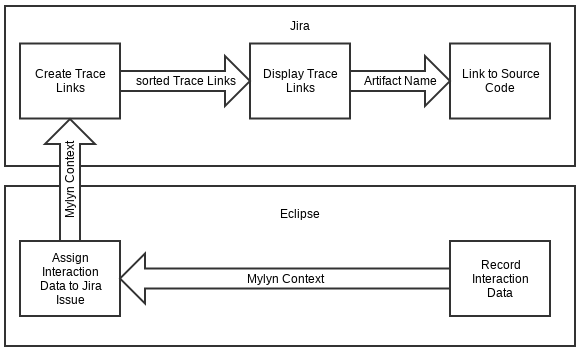
\includegraphics[width=.9\linewidth]{images/Approach-Flowchart.png}
	\caption{Some random image I had lying around in another \LaTeX\  report.}
	\label{fig:random_image}
\end{figure}

Here is me talking about figure \ref{fig:random_image}.

\begin{figure}[!htb]
	\centering
	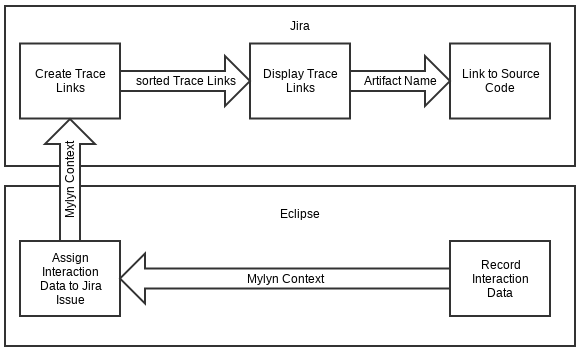
\includegraphics[width=.4\linewidth]{images/Approach-Flowchart.png}
	\quad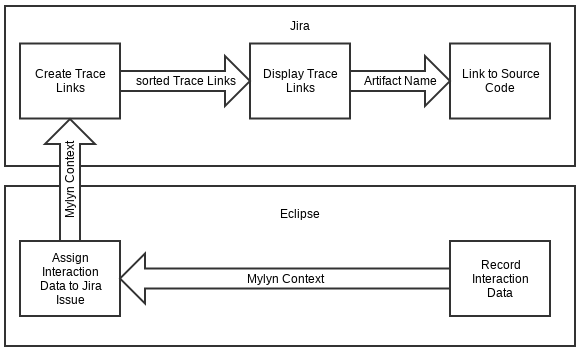
\includegraphics[width=.4\linewidth]{images/Approach-Flowchart.png}
	\caption{This is getting out of hand! Now there is two of them!}
	\label{fig:lolnooneevenusesthisimage}
\end{figure}


Look at table \ref{tab:somerandomtablethatshouldnotbehere}, it's all shiny and without lines boxing it in on all sides. Or you can just draw a sudoku, see if I care.


\begin{center}
\begin{tabular}{ p{\textwidth /4}  p{\textwidth *3 /5 }}

	Description & The way developers approach a task can provide detailed information about the structure of the project they are working on.
	Using this knowledge, other team-members can familiarize themselves with new parts of the project faster.
	This information can be displayed as trace links, which show the source code entities, that are relevant to a particular requirement specification.
	While the users can benefit from these trace links, their creation should not interfere with the normal workflow. Why is this even still on my hard-drive, I handed it in years ago.\\
	\hline
	User Subtasks & User Subtask 1.1: perform interactions\\
	& User Subtask 1.2: commit changes related to an issue\\
	& User Subtask 1.3: browse linked code entities\\	
\end{tabular}
	\label{tab:somerandomtablethatshouldnotbehere}
\captionof{table}{If you don't add a caption, the table wont show up in the list of tables. I invested a lot of clicks into making that, so you better think of something clever to put there.}
\end{center}

Notice how this tabular doesn't float all over the place? use regular tables if you prefer it that way.
\chapter{Conclusion}
by Patrick Dammann

\bigskip

In this project, several methods for music genre classification have been tested. While the first part focussed on handling the raw signal of the song with a specially designed neural network, the following two parts concentrated on good preprocessing and models that are designed to handle it.

Since the dataset was heavily imbalanced, our results can't be directly compared, for accuracies up to $~68$\% can be achieved by ignoring $13$ of the $16$ genres completely. The imbalance of the dataset therefore also heavily influenced our training, since a high bias on frequent labels should be the easiest and most promising direction for the network to follow to obtain low losses. In the end that also means that our results are not very meaningful.

\section{Future Attempts}
First and foremost, future research need a more structured dataset. Since we wanted to perform better than previous attempts on this problem, one of our initial intents was to use more data, which seemed to be simple with the enormous dataset we found. Being way to enthusiastic about the dataset we forgot to check whether there could be errors in it, since it seemed to be well preprocessed by its offerers. With the empty label removed from the beginning, we could have saved much time on unnecessary work and trainings.

The imbalance of the dataset turned out to be a way bigger problem than we initially thought. While we first thought about the bias in the set as a wanted bias, since a big archive like the FMA might resemble the real-world-distribution of music, we soon learned that out models mainly concentrated on learning a bias than on learning general classification qualities.

With a new dataset, other improvements could be realized. For example, the combination of individual models. Especially the pre-processed data of the entropy attempt can easily be fed into another network, maybe helping it by erasing the need to generate similar features itself or by boosting classification by adding a dimension where the data can be more easily separated.

Also, we often copied and sometimes guessed hyper-parameters. These could have been optimized via gaussian processes, or more advanced algorithms like the one provided by \emph{pytorch} used for the entropy approach.
Unfortunately, these optimizations cost a great amount of time for networks with a higher forward- and backward-pass time and of course a higher number of hyper-parameters.
%% Bibliography
% natbib style, requires the usage of natbib: \bibliographystyle{plainnat}
\bibliographystyle{is-alpha}
\bibliography{literature}%Bibliography file name

\listoffigures

\listoftables

\end{document}          
